\documentclass[10pt]{article}
\usepackage[frenchb,english]{babel}
\usepackage{multirow}
\usepackage{graphicx}
\usepackage{calc}
\usepackage{caption}
\usepackage{array}
\usepackage{booktabs}
\usepackage{amsmath}
\usepackage{rotating}
\usepackage{tikz}
\usepackage{tabularx}
\usepackage{booktabs}
\usetikzlibrary{positioning,calc}
\newcommand{\defineWidthHeight}[2]{

\newcounter{margin}
\newcounter{Paperwidth}
\newcounter{Paperheight}

\setcounter{margin}{2}
\setcounter{Paperwidth}{#1}
\setcounter{Paperheight}{#2} 

\usepackage[margin=\themargin mm]{geometry}
\setlength{\paperwidth}{\thePaperwidth mm} 
\newcounter{Textwidth}
\setcounter{Textwidth}{\value{Paperwidth}-2*\value{margin}}
\setlength{\textwidth}{\value{Textwidth} mm}
\setlength{\paperheight}{\thePaperheight mm} 
\newcounter{Textheight}
\setcounter{Textheight}{\value{Paperheight}-2*\value{margin}}
\setlength{\textheight}{\value{Textheight} mm}
\setlength{\parindent}{0mm}
}
\fontfamily{phv}\selectfont
\setlength{\parindent}{0cm}
%%%%%%%%%%%%%%%%%%%%%%%%%%%%%%%%%%%%%%%%%%%%%%%%%%%%%%%%%%%%%%%%%%%%%%%%%
% Command to automatically crop the pdf file
%%%%%%%%%%%%%%%%%%%%%%%%%%%%%%%%%%%%%%%%%%%%%%%%%%%%%%%%%%%%%%%%%%%%%%%%%
\newcommand\cropped[2]{%
    \immediate\write18{pdfcrop #1.pdf #1_cropped.pdf}%
    \includegraphics[width=#2\textwidth]{#1_cropped.pdf}}
%%%%%%%%%%%%%%%%%%%%%%%%%%%%%%%%%%%%%%%%%%%%%%%%%%%%%%%%%%%%%%%%%%%%%%%%%
\defineWidthHeight{190}{140}
\usepackage[percent]{overpic}

\begin{document}
\fontfamily{phv}\selectfont
\def\raiseS[#1]{\raisebox{2\height}{#1}}
\def\coll{0.45\textwidth}
\def\up{3.5}
%-----------------------------------------------------------------------------------------------------------------------------------------------------------------------
% Set path of  code here (i.e. where plots are exported)
%-----------------------------------------------------------------------------------------------------------------------------------------------------------------------
\graphicspath{
{../../code/}
}	
%-----------------------------------------------------------------------------------------------------------------------------------------------------------------------
\begin{tabular}{c|c}
\textbf{ Clinico-biologico-radiological}
&
\textbf{ Clinico-biologico-radiological + mathematical}
\\[2mm]
\begin{overpic}[width=\coll]{cox_regression/os/hazard_ratios_all_features} 
%  \put (65, 30) {\textbf{c-index = 0.675}}
  \put (-5, 68) {\textbf{A}}
\end{overpic}
& 
\begin{overpic}[width=0.52\textwidth]{mechanistic/cox_regression_mechanistic_clinical/os/hazard_ratios_all_features} 
%  \put (70, 26) {\textbf{c-index = 0.733}}
  \put (0, 58) {\textbf{B}}
\end{overpic}
\end{tabular}
\vskip1cm
\raisebox{5cm}{\textbf{C}} \hspace{0.2cm}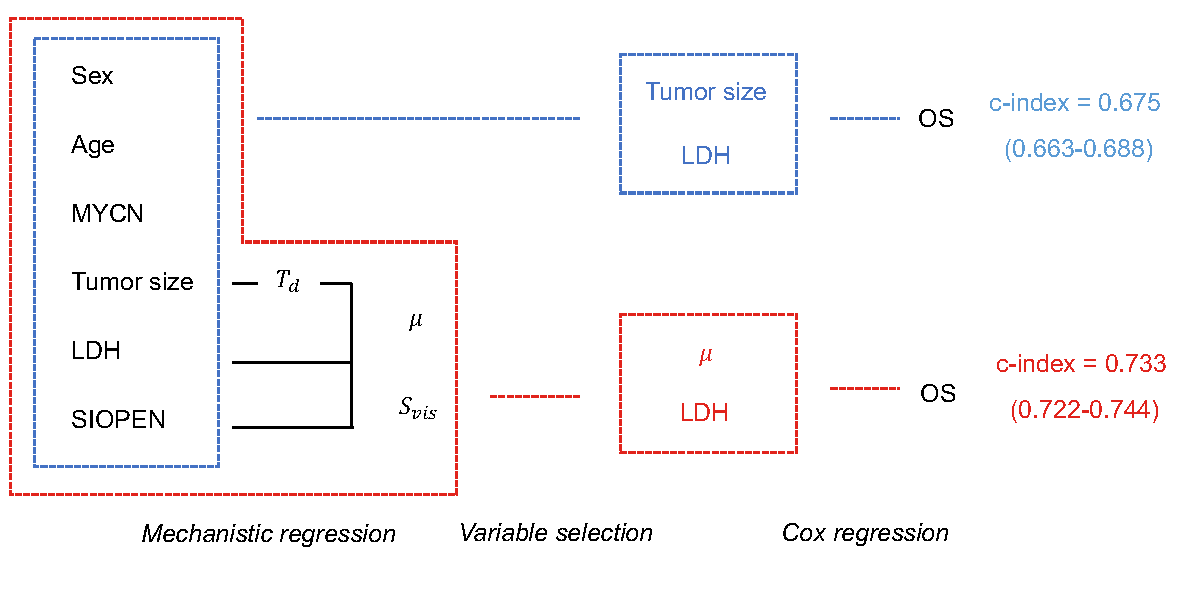
\includegraphics[width=0.6\textwidth]{regression}
%\\
%\vskip0.4cm
\raisebox{4cm}{\textbf{D}} \hspace{0.2cm}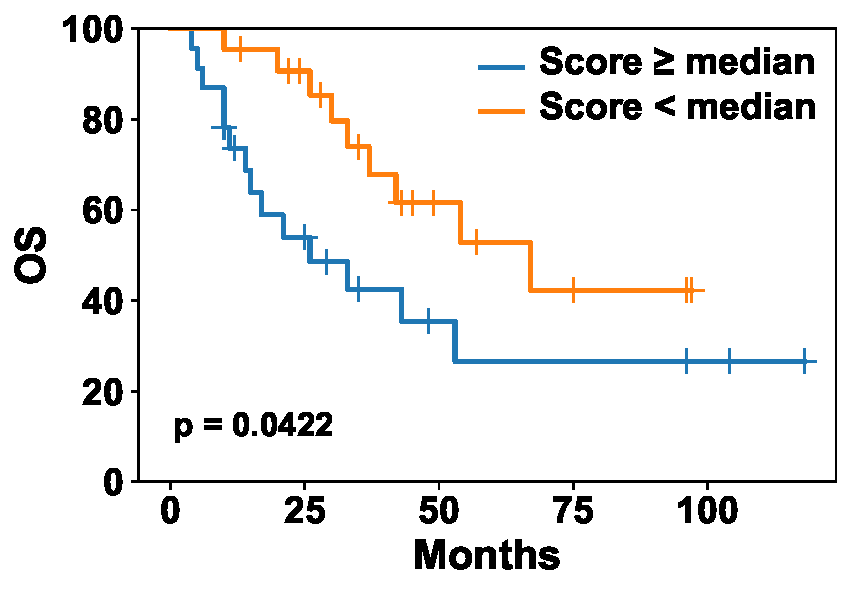
\includegraphics[width=0.35\textwidth]{mechanistic/cox_regression_mechanistic_clinical/os/separation_cox_score}
\end{document}